\subsection{Anzeigen einer Polyline}
\label{sub:anzeigen_einer_polyline}
  Zu beginn stellte sich die Frage, wie sich in kleinen Schritten an das komplexe Thema einer Live Visualisierung ran getastet werden kann. Die erste Hürde ist die Animation von nur \textbf{einem} Vehicle entlang einer Polyline. Die Umsetzung davon, soll in diesem und den nächsten zwei Abschnitten \ref{sub:hinzufügen_der_stationen} und \ref{sub:animieren_eines_vehicles_durch_interpolation} erklärt werden.

  Um eine Datengrundlage zu haben wurde ein möglichst vollständiges GTFS-Feed aus \texttt{TransitFeeds.com} ausgewählt und in die Datenbank importiert. Die Wahl fiel dabei auf das Boston-MBTA Feed. Die Herausforderung bestand nun darin, erste Daten aus der Datenbank an den Client zu senden und sie dort darzustellen. Fast trivial ist das Abfragen der Polyline: \colorbox{lightGrey}{\texttt{\color{white}{{\color{materialBlue} SELECT} * {\color{materialBlue}FROM} gtfs\_shapes {\color{materialBlue}WHERE} shape\_id = {\color{materialRed}12345}}}}

  \begin{figure}[htbp]
    \begin{center}
      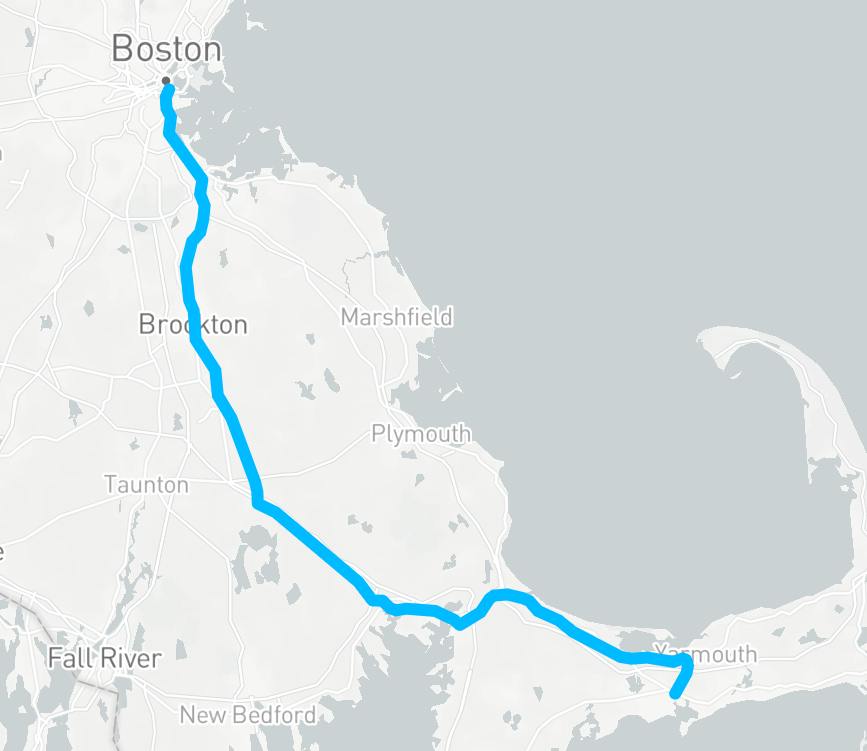
\includegraphics[width=0.5\textwidth]{prozess/draw_single_shape}
      \caption{Anzeigen einer einzigen Polyline in Boston}
      \label{fig:prozess/draw_single_shape}
    \end{center}
  \end{figure}
  
  Die Daten der Polyline werden als GeoJSON übertragen und lassen sich mittels Mapbox-gl-js auf der Karte anzeigen. Abbildung \ref{fig:prozess/draw_single_shape} zeigt das Ergebnis dieser ersten Iteration. Zu sehen ist bereits die Karte mit der Polyline (hier in blau). Die Abgefragten Daten können also nun bereits verarbeitet und angezeigt werden. Damit ein Vehicle entlang dieser Linie animiert werden kann, werden die einzelnen Stationen des Trips benötigt.
  Dieser ständige Wechsel zwischen der Arbeit am Backend um neue Datenabfragen zu ermöglichen und dem Frontend um diese anschließend Anzuzeigen, stellte sich als sehr effektiv heraus und zog sich durch das gesamte Projekt hinweg durch.
% subsection anzeigen_einer_polyline (end)